\documentclass[xcolor=table]{beamer}
%%%https://github.com/hdante/picat-lang/blob/master/doc/predfunc.tex
%\documentclass[10pt]{beamer} 
%\usetheme[pageofpages=of,% String used between the current page and the
          % total page count.
%          alternativetitlepage=true,% Use the fancy title page.
          %titlepagelogo=coca,% Logo for the first page.
%          titleline=true
%          ]{chameleon}
%\usetheme{Frankfurt}


\mode<presentation> {

% The Beamer class comes with a number of default slide themes
% which change the colors and layouts of slides. Below this is a list
% of all the themes, uncomment each in turn to see what they look like.

%\usetheme{default}
%\usetheme{AnnArbor}
%\usetheme{Antibes}
%\usetheme{Bergen}
%\usetheme{Berkeley}
%\usetheme{Berlin}
%\usetheme{Boadilla}
%\usetheme{CambridgeUS}
%\usetheme{Copenhagen}
%\usetheme{Darmstadt}
%\usetheme{Dresden}
%\usetheme{Frankfurt}
%\usetheme{Goettingen}
%\usetheme{Hannover}
%\usetheme{Ilmenau}
%\usetheme{JuanLesPins}
%\usetheme{Luebeck}
%\usetheme{Madrid}
%\usetheme{Malmoe}
%\usetheme{Marburg}
%\usetheme{Montpellier}
%\usetheme{PaloAlto}
\usetheme{Pittsburgh}
%\usetheme{Rochester}
%\usetheme{Singapore}
%\usetheme{Szeged}
%\usetheme{Warsaw}

% As well as themes, the Beamer class has a number of color themes
% for any slide theme. Uncomment each of these in turn to see how it
% changes the colors of your current slide theme.

%\usecolortheme{albatross}
%\usecolortheme{beaver}
%\usecolortheme{beetle}
%\usecolortheme{crane}
%\usecolortheme{dolphin}
%\usecolortheme{dove}
%\usecolortheme{fly}
%\usecolortheme{lily}
%\usecolortheme{orchid}
%\usecolortheme{rose}
%\usecolortheme{seagull}
%\usecolortheme{seahorse}
\usecolortheme{whale}
%\usecolortheme{wolverine}

%\setbeamertemplate{footline} % To remove the footer line in all slides uncomment this line
%\setbeamertemplate{footline}[page number] % To replace the footer line in all slides with a simple slide count uncomment this line

%\setbeamertemplate{navigation symbols}{} % To remove the navigation symbols from the bottom of all slides uncomment this line
}


%\usecolortheme{chameleon}

\usepackage{graphicx,hyperref,url}
\usepackage[utf8]{inputenc}
\usepackage[T1]{fontenc}
\usepackage[portuges,brazilian]{babel}
%%%\usepackage{wrapfig}
\usepackage{caption}
\usepackage{subfigure}
%\usepackage{subcaption}
\usepackage{latexsym}
\usepackage{amssymb, amsmath}
\usepackage{multicol}
\usepackage{pifont}%,bbding}%%,dingbat} %%% ver manual de simbolos
\usepackage[final]{listings}
\usepackage{comment}
\usepackage[misc]{ifsym}
\usepackage{array}
\usepackage{blindtext}
\usepackage{lipsum}
%\usepackage{enumitem} ====> NEVER 
%\usepackage[table,xcdraw]{xcolor}

\setbeamertemplate{caption}[numbered]

\definecolor{azulclaro}{rgb}{0.9,0.9,0.9}
\definecolor{mygreen}{rgb}{0,0.6,0}
\definecolor{mygray}{rgb}{0.5,0.5,0.5}
\definecolor{mymauve}{rgb}{0.58,0,0.82}
\definecolor{darkgray}{rgb}{.4,.4,.4}
\definecolor{purple}{rgb}{0.65, 0.12, 0.82}

%\newcommand{\minizinc}{MiniZinc}

\newenvironment{CustomBlock}[3]{%
	\setbeamercolor{block body}{#2}
	\setbeamercolor{block title}{#3}
	\begin{block}{#1}}{\end{block}}

\lstset{ 
  %  label={pgm_ex01},
    backgroundcolor=\color{azulclaro}, 
    language=erlang, %%Miranda,%%Perl,%%%Python, %%Mercury,
    showstringspaces=false,
    basicstyle=\bf\scriptsize\ttfamily,
%%      basicstyle= \footnotesize %%% TESTAR
%%      keywordstyle=\bfseries\color{green!40!black},
    keywordstyle=\textbf{\color{mygreen}}, 
    otherkeywords={*, \%, array, constraint, solve, output,  show, "/\", satisfy, set, of, if, then, elseif, float, search},
%%  keywordstyle=\color{blue},       % keyword style
%%    commentstyle=\itshape\color{purple!40!black},
      commentstyle=\color{orange},    % comment style
      identifierstyle=\color{blue},
      stringstyle=\color{orange},
      stringstyle=\color{mymauve},
      numbers=left,  % where to put the line-numbers; possible values are (none, left, right)
      numbersep=5pt,   % how far the line-numbers are from the code
      numberstyle=\tiny\color{magenta},
      keepspaces=true      
    % %caption={LEGENDA no source PASCAL ficou OK},
}


\graphicspath{{/home/ccs/Dropbox/figs_genericas/}{figuras/}{figures/}}
\DeclareGraphicsExtensions{.pdf,.png,.jpg}
%Global Background must be put in preamble
%\usebackgroundtemplate{\includegraphics[width=\paperwidth]{amarelinho.pdf}}
%%% \begin{frame}[allowframebreaks=0.8]

% The log drawn in the upper right corner.

\logo{\centering
%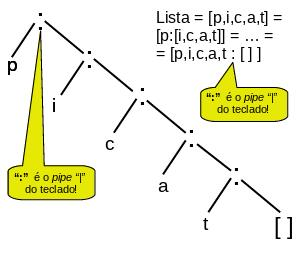
\includegraphics[height=0.10\paperheight]{figures/logo01-picat.jpg}

\includegraphics[height=0.11\paperheight]{figures/logo02-picat.jpg}
\hspace{0.9\paperwidth}
%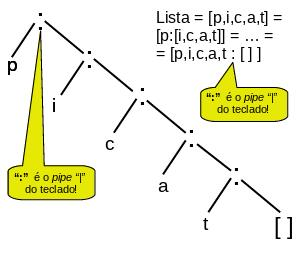
\includegraphics[height=0.027\paperheight]{figures/logo01-picat.jpg}
}

%%%%%%%%%%%%%%%%%%%%%%%%%%%%%%%%%%%%%%%%%%%%%%%%%%%%%%%%%%%%%%%%%%%%%

\title[Picat]{\fontsize{20}{30}\selectfont \textcolor{black}{PICAT: Uma Linguagem de Programação Multiparadigma\\
Usando o Modulo \textit{planner}}}

\author[Claudio Cesar de Sá]{Claudio Cesar de Sá
\\\medskip 
\Letter \/ {\small \url{ccs1664@gmail.com}}\\
\Letter \/ {\small \url{ccs1664@yahoo.com}}
}

\institute[]{
    Pesquisador Independente \\
    \url{https://claudiocesar.wordpress.com/}

}

%%%%%%%%%%%%%%%%%%%%%%%%%%%%%%%%%%%%%%%%%%%%%%%%%%%%%%%%%%%%%%%%%%%%%

\begin{document}
\begin{frame}
    \titlepage
\end{frame}

%%%%%%%%%%%%%%%%%%%%%%%%%%%%%%%%%%%%%%%%%%%%%%%%%%%%%%%%%%%%%%%%%%%%%
% \include{aula_apresentacao_curso_picat}
% %%%%%%%%%%%%%%%%%%%%%%%%%%%%%%%%%%%%%%%%%%%%%%%%%%%%%%%%%%%%%%%%%%%%%
%
  \begin{frame}[allowframebreaks,c]{Sumário}
   \tableofcontents
  \end{frame}
% %%%%%%%%%%%%%%%%%%%%%%%%%%%%%%%%%%%%%%%%%%%%%%%%%%%%%%%%%%%%%%%%%%%%%
%%%%%%%%%%%%%%%%%%%%%%%%%%%%%%%%%%%%%%%%%%%%%%%%%%%%%%%%%%%%%%
\section{Introdução}


%%%%%%%%%%%%%%%%%%%%%%%%%%
\begin{frame}
\frametitle{Introdução}
\begin{minipage}{0.47\textwidth}
    \begin{itemize}
        \item Histórico
        \item Contexto
        \item Exemplo: \textit{Alo Mundo}
        \item Como usar
    \end{itemize}
\end{minipage}
\begin{minipage}{0.5\textwidth}
\begin{figure}[ht!]
\begin{center}

\includegraphics[width=1.2\textwidth, height=0.40\textheight]{figures/logo_picat_alex.jpg}
\end{center}
\end{figure}
\end{minipage}
\end{frame}
%%%%%%%%%%%%%%%%%%%%%%%%%%



\begin{frame}

    \frametitle{Histórico}

    \begin{itemize}
      \item Criada em 2013 por Neng-Fa Zhou e Jonathan Fruhman -- USA

      \item Utiliza o B-Prolog (Neng-Fa Zhou) como base de implementação, tendo
      a Lógica de Primeira-Ordem (LPO) como parte de seu mecanismo programação

\pause
      \item Uma evolução ao Prolog após seus mais de 40 anos de sucesso!

\pause
      \item Sua atual versão é a 2.x (\today).
\pause
      \item Código-aberto, segue as regras da FSF

    \end{itemize}
\end{frame}

%%%%%%%%%%%%%%%%%%%%%%%%%%%%%%%%%%%%%%%%%%%%%%%%%%%%%%%%%%%%%%%%%%%%%

\begin{frame}[fragile]
  \frametitle{Links do PICAT}

  \begin{itemize}
   	\item Site oficial: \textbf{\textcolor{violet}{\url{http://picat-lang.org}}} -- links, forum, livro, videos etc

   	\item Site do Hakan -- Suécia:  \url{http://www.hakank.org/picat/}

  \item   \textbf{Videoaula 01: Introdução ao PICAT}, disponível no Youtube:\\
    \textbf{\url {https://www.youtube.com/watch?v=0DmTyFFQPK8}}

   \item   \textbf{Videoaula 02: Introdução ao PICAT}, disponível no Youtube:\\
  \textbf{\url {https://www.youtube.com/watch?v=7fPKPd0ZDnc}}

   \item   \textbf{Videoaula: Depuração com PICAT}, disponível no Youtube:\\
  \textbf{\url {https://www.youtube.com/watch?v=9axovyzMqwc}}

    
   	\item Editor on-line mantido pelo Alexandre: \url{http://retina.inf.ufsc.br/picat.html}
     
    
    \item Se não tiver \textit{plugin} para Picat, escolha a sintaxe da linguagem \textit{Erlang}.
    
  \end{itemize}

\end{frame}

%%%%%%%%%%%%%%%%%%%%%%%%%%%%%%%%%%%%%%%%%%%%%%%%%%%%%%%%%%%%%%%%%%%%%



\subsection{Estrutura da Linguagem}

\begin{frame}
	\frametitle{Conhecendo PICAT}
    
    \begin{itemize}
    
    	\item Picat é uma linguagem de programação simples de usar, poderosa e multi-uso
        
        \item Alguma de suas características 
         são associadas com linguagens lógicas, como Prolog, B-Prolog, Goedel, etc
        
        \pause
        \item Picat é uma linguagem essencialmente multiparadigma,
        abrangendo partes de vários paradigmas de programação: declarativo (lógico e funcional) e     imperativo
        
        %\item Esta combinação de características declarativas e imperativas permite
        %o desenvolvimento de softwares mais produtivos, mas que ainda possam ser altamente 
        %otimizados para tarefas específicas, ou softwares mais simples para tarefas mais mundanas;
        
    \end{itemize}
    
\end{frame}

%%%%%%%%%%%%%%%%%%%%%%%%%%%%%%%%%%%%%%%%%%%%%%%%%%%%%%%%%%%%%%%%%%%%%

\begin{frame}[fragile]
    \frametitle{O que é ser Multiparadigma ?}

    \begin{itemize}
    
    \item Paradigma: um conjunto de características baseado em alguma abordagem teórica 
    
    \pause
      \item Picat é uma linguagem multiparadigma pois abrange os seguintes paradigmas:
    
      \begin{itemize}
      	\item[--] Lógico
      	\item[--] Funcional
      	\item[--] Procedural
      \end{itemize}
      
     \pause
      \item Em resumo,  \textit{uma boa mistura} de: Haskell (Funcional) , Prolog (Lógica) e 
      Python (Procedural e Funcional).
      
    \end{itemize}
      
\textbf{\textcolor{red}{Pular .... leiam com calma, depois!}}
\end{frame}

%%%%%%%%%%%%%%%%%%%%%%%%%%%%%%%%%%%%%%%%%%%%%%%%%%%%%%%%%%%%%%%%%%%%%
\subsubsection{Paradigmas}
\begin{frame}[fragile]
	\frametitle{Paradigma Lógico}
    
    \begin{itemize}
    
    	\item Uma linguagem lógica é uma onde o programa é expresso como um conjunto
        de predicados lógicos, escritos por \textit{fatos} e \textit{regras}
    
    \pause
    	\item Regras são escritas em formas de cláusulas, as quais são interpretadas como
        implicações lógicas.\\ 
        Dependem das premissas serem verdadeiras para esta ser verdadeira.
        

    \pause
    	\item Fatos são cláusulas sem premissas, verdades absolutas.

        
        \pause
        \item Este   paradigma é a  \textbf{base} do Picat
    \end{itemize}

\end{frame}

%%%%%%%%%%%%%%%%%%%%%%%%%%%%%%%%%%%%%%%%%%%%%%%%%%%%%%%%%%%%%%%%%%%%%

\begin{frame}[fragile]
	\frametitle{Paradigma Funcional}
    
    \begin{itemize}
    
    
    	\item Uma linguagem funcional é uma onde os elementos do programa podem ser avaliados e 
        tratados como funções matemáticas.
        
        \pause
         \item Um dos principais motivos em usar linguagens funcionais é a previsibilidade
         e facilidade no entendimento do estado atual do programa.
         
         \pause
         \item Este fato de uma  sintaxe simples, torna o Picat  intuitivo e legível na
         funcionalidade de seus códigos.
         
    \end{itemize}
    
    
\end{frame}

%%%%%%%%%%%%%%%%%%%%%%%%%%%%%%%%%%%%%%%%%%%%%%%%%%%%%%%%%%%%%%%%%%%%%

\begin{frame}[fragile]
	\frametitle{Paradigma Procedural}
    
    \begin{itemize}
    
    	\item Uma linguagem procedural é uma que pode ser subdividida em \textit{procedimentos},
        também chamados de rotinas, subrotinas ou funções
        
        \pause
        \item Em linguagens procedurais há um procedimento principal (em geral é chamado de 
        \textit{Main}) que controla o uso e a chamada de outros procedimentos. Em Picat há
        tal hierarquia.
        
        \pause
        \item Em Picat, cada premissa é tratada como um procedimento, que é resolvido por meio
        de métodos de inferência lógica.
       
    \end{itemize}
    
\framebreak
    
    \begin{figure}
    	\begin{columns}
    		\column{.6\linewidth}
	         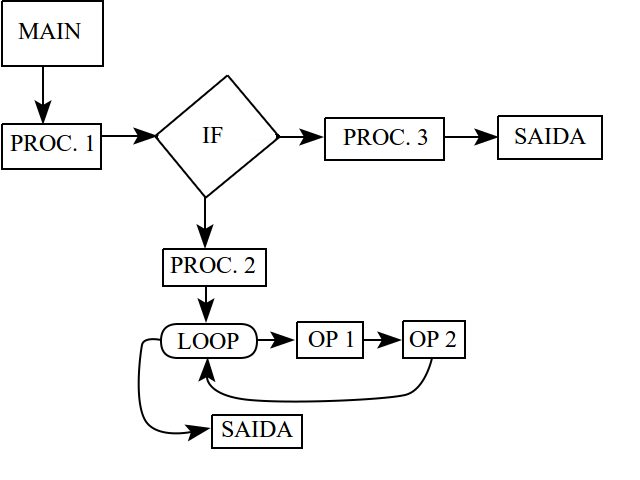
\includegraphics[width=.8\textwidth] {figures/Paradigma_Procedural.png}
             \column{.4\linewidth}
             \caption{Fluxograma representando a estrutura de um programa Procedural}
	         \label{Fluxograma Procedural}
		\end{columns}
	\end{figure}

\textbf{\textcolor{red}{Retomar aqui ...}}    
\end{frame}

%%%%%%%%%%%%%%%%%%%%%%%%%%%%%%%%%%%%%%%%%%%%%%%%%%%%%%%%%%%%%%%%%%%%%

\begin{frame}[fragile]
    \frametitle{Algumas Características:}


    \begin{itemize}
    
    \pause 
      \item Sintaxe elegante e simples, facilitando a leitura e entendimento do código
      
          \pause 
      \item Velocidade de execução em um ambiente \textit{interpretado} (há
      uma \textit{máquina
      virtual} como Python, Java e alguns Prologs)
      
          \pause 
      \item Disponibilidade em vários sistemas operacionais e arquiteturas
      
      \pause 
      \item Análogo a Python, podem ser feitas \textit{queries}
      ou \textit{consultas} ao terminal de Picat.

      \pause 
      \item Há várias bibliotecas da própria linguagem, e diversas ferramentas
      externas permitindo o incremento do poder do Picat.
      
    \end{itemize}
\end{frame}

%%%%%%%%%%%%%%%%%%%%%%%%%%%%%%%%%%%%%%%%%%%%%%%%%%%%%%%%%%%%%%%%%%%%%


\begin{frame}	 [fragile]

   \frametitle{Acrônimo de \textbf{P.I.C.A.T.}}
  
  
  \begin{block}{}
  		\begin{description}

 \item [\textbf{P}:] \textit{Pattern-matching}:  Utiliza o conceito de \textit{casamento de 
padrões} entre objetos, bem como os conceitos da \textit{unificação} da LPO

\item [\textbf{I}:] \textit{Intuitive}: Oferece estruturas de decisão, atribuição e laços de
repetição, etc. Análogo há outras linguagens de programação mais populares

\item [\textbf{C}:] \textit{Constraints}: Suporta a programação por restrições (PR) para 	
problemas combinatórios

 \item [\textbf{A}:] \textit{Actors}: Suporte as chamadas a eventos, chamada via \textit{atores}

\item [\textbf{T}:] \textit{Tabling}: Implementa a técnica de \textit{memoization} com 
soluções imediatas para problemas de Programação Dinâmica (PD).

  \end{description}	
 \end{block}
  
\end{frame}


%%%%%%%%%%%%%%%%%%%%%%%%%%%%%%%%%%%%%%%%%%%%%%%%%%%%%%%%%%%%%%%%%%%%%

\subsubsection{Usando Picat}

\begin{frame}[fragile]
  \frametitle{Usando Picat}
  	\begin{itemize}
    
    % \item Picat é uma linguagem  disponível em qualquer arquitetura de 
    % processamento. 
      
    %\pause
    %\item Qualquer emergência, o ambiente completo de execução do Picat pode ser reconstruído a partir da linguagem C padrão
      
   
      \item Os seus arquivos fontes utilizam a extensão \textbf{.pi}. Exemplo: \texttt{programa.pi}
      \item Há dois modos principais de utilização do Picat: 
      
      \begin{itemize}
      	\item[--] Modo interativo, onde seu código é digitado e compilado diretamente na linha de 
        comando;
      	\item[--] \textit{Modo console} onde o console só é utilizado para compilar seus programas.
      \end{itemize}
      
      \pause
      \item Códigos executáveis 100\% \textbf{stand-alone}: ainda não!
      \item Neste quesito, estamos em igualdade com Java, Prolog e Python
     
    \end{itemize}
\end{frame}





\begin{frame}[fragile]
\frametitle{Exemplo -- \textit{Alô Mundo!}}

Acompanhar as explicações do código de:\\
\url{https://github.com/claudiosa/CCS/blob/master/picat/alo_mundo.pi}

\begin{verbatim}
main => msg_01  , 
        msg_02 .
        
msg_01 =>  printf("  ALO MUNDO!!! ").
msg_02 =>  printf("\n  FIM \n").
\end{verbatim}

\end{frame}


\begin{frame}[fragile]
\frametitle{Execução na Console Linux ou Windows}

\begin{verbatim}
$ picat alo_mundo.pi 
  ALO MUNDO!!! 
  FIM 
$ 
\end{verbatim}

\pause
\textcolor{red}{Análogo ao desenvolvimento com Python!}

\end{frame}


\begin{frame}[fragile]
\frametitle{Execução no Ambiente do Interpretador}

\begin{footnotesize}
\begin{verbatim}
$ picat
Picat 2.0, (C) picat-lang.org, 2013-2016.
Type 'help' for help.
Picat> cl(álo_mundo.pi').
Compiling:: alo_mundo.pi
alo_mundo.pi compiled in 0 milliseconds
loading...

yes

Picat> main 
  ALO MUNDO!!! 
  FIM 

yes

Picat> msg_02

  FIM 

yes

Picat> 
\end{verbatim}

\end{footnotesize}
\end{frame}


\begin{frame}[fragile]
\frametitle{Ambiente do Interpretador -- Uso do \texttt{getline}}

\textbf{\textcolor{red}{Saltar aqui ... depois leiam com calma!}}  

\begin{itemize}
  \item Inicialmente, aqui o código foi carregado com o comando `\texttt{cl}' (digite \texttt{help} na console), o qual \textbf{compila} o seu código e \textbf{carrega} em um código intermediário pronto
  para ser executado e testado
  
  \pause
  \item Neste ambiente interpretado há comandos básicos de teclado (mouse não funciona aqui)
  do programa \texttt{getline} do Linux. Os mais importantes são:
  \pause
  \begin{itemize}
    \item  \textbf{Crtl-a}: move o cursor para o início da linha
        \item  \textbf{Crtl-e}: move o cursor para o final da linha (\textit{end})
        \item  \textbf{Crtl-f}: 	move o cursor de uma posição a frente (forward)
         \item  \textbf{Crtl-b}: 	move o cursor de uma posição para trás (backward)
         \item  \textbf{Crtl-d}: 	exclui o carácter sob  o cursor (a 2a. vez -- sai do ambiente)
        \item  \textbf{Crtl-u}: 	exclui a linha inteira
        \item As flechas ... repetem os últimos comandos
  \end{itemize}
  
\end{itemize}

\end{frame}



\begin{frame}[fragile]
\frametitle{Ambiente do Interpretador -- Uso}

\begin{itemize}
  \item Use um editor externo de sua preferência. Por exemplo:
   \texttt{geany} com plugin do Picat

    \pause
  \item Mantenha duas janelas de terminais abertas
    \begin{itemize}
    \item Uma para o ambiente interpretado
    \item Outra para usá-lo diretamente: \texttt{\$console\$ picat seu\_programa.pi}
  \end{itemize}
  
    \pause
  \item Os dois modos são importantes de se trabalhar simultaneamente
  
  \pause
  \item Em dúvidas, digite: \texttt{Picat> help .}
    
\end{itemize}

\end{frame}


\begin{frame}[fragile]
\frametitle{Reflexões}

\begin{itemize}



      \pause
      \item Para próxima seção esteja com o Picat instalado em seu 
      computador para um melhor aproveitamento.
    \pause

  \item Em códigos fontes: o símbolo '\%' no início de linha, comenta a linha  corrente

\end{itemize}

\textbf{\textcolor{red}{Retomar aqui ...}}  
\end{frame}

%%%%%%%%%%%%%%%%%%%%%%%%%%%%%%%%%%%%%%%%%%%%%%%%%%%%%%%%%%%%%%%%%%%%%

 \section{Planejamento}


%%%%%%%%%%%%%%%%%%%%%%%%%%
\begin{frame}
\frametitle{Planejamento}
\begin{minipage}{0.47\textwidth}
    \begin{itemize}
        \item O que é Planejamento?
        \item Importância da área
        \item Muitas definições
        \item Exemplo
    \end{itemize}
\end{minipage}
\begin{minipage}{0.5\textwidth}
\begin{figure}[ht!]
\begin{center}

\includegraphics[width=1.2\textwidth, height=0.40\textheight]{figures/logo_picat_alex.jpg}
\end{center}
\end{figure}
\end{minipage}
\end{frame}
%%%%%%%%%%%%%%%%%%%%%%%%%%

\begin{frame}[fragile]
%[fragile, allowframebreaks=0.9]

 \frametitle{Planejamento}

   \begin{block}{}
     \begin{itemize}
      \item Requisitos: recursividade, listas e PD
       \pause
      
      \item Além destes: conceitos grafos, árvores de busca, nós, etc
       
       \pause
      \item \textit{Planejamento} é um \textcolor{magenta}{\textbf{termo amplo e em vários domínios}} 
      
       \pause
      \item \textcolor{red}{O que \textbf{não} é o nosso contexto de \textit{planejamento}?}\\
      Exemplo: planejamento estratégico das empresas, planejar como distribuir
      os dividendos da empresa, orçamento familiar,  etc
      
      \pause
       \item \textcolor{violet}{O que é o nosso contexto de \textit{planejamento}?}
       \pause
       Questões que envolvam um ambiente, um agente (um programa, um robô, etc), sensores,
      e ações que modifiquem estados.\\ Exemplo clássico:  robótica em geral
 
    \end{itemize}
    
    \end{block}
    
\end{frame}



\begin{frame}[fragile]
%[fragile, allowframebreaks=0.9]

    \frametitle{Planejamento}

   \begin{block}{}
     \begin{itemize}
 
       
      \item Problemas em geral necessitam de um \textcolor{magenta}{\textbf{plano}} 
      para serem solucionados, assim,
      há uma visão que encontrar um plano para um problema $\Rightarrow$ ter uma solução!

      \pause
      \item Em resumo, a área de planejamento é bem complexa, 
       antiga na área da IA e robótica (1970 -- STRIPS), 
       efervescente, e de muito interesse na indústria.
           
      \pause
      \item Várias abordagens sobre a visão clássica da IA. Mas temos evoluções
      significativas ...
      
      \pause
      \item PDDL (\textit{Planning Domain Definition Language}): unanimidade (ou próxima a esta)
      entre os pesquisadores de planejamento, como linguagem descritora
      de problemas de planejamento.

      \pause
      \item Vários problemas ainda sem solução, pois a complexidade é exponencial 
      
      
     %  \pause
      
%     \item 

    \end{itemize}
    
    \end{block}
    
\end{frame}



\begin{frame}[fragile]
%[fragile, allowframebreaks=0.9]

  \frametitle{Definições}

   \begin{block}{}
     \begin{itemize}
      \item Plano: seqüência ordenada de ações
       \pause
         \begin{itemize}
           \item problema: escalar o Everest, comprar um abacate, leite e uma furadeira (nesta ordem)

           \pause
            \item plano: ir ao supermercado, ir à seção de frutas, pegar as bananas, 
            ir à seção de leite, pegar uma caixa de leite, ir ao caixa,  pagar tudo, 
            ir a uma loja de ferramentas, ..., voltar para casa.
                                
         \end{itemize}

       \pause
       \item Um Planejador:
        Combina conhecimento de um ambiente, um agente e suas ações possíveis,
        entradas (luz, cor, cheiro, sensor, etc), um estado corrente
        e/ou inicial, e com isto resolve de problemas planejar sequência
        de ações, que mudam de estados a cada ação, até atingir um 
        estado final.
       
    \end{itemize}
    
    \end{block}
    
\end{frame}



\begin{frame}[fragile]
\frametitle{Exemplos do que é planejamento ...}

\begin{figure}[!htb]
\centering
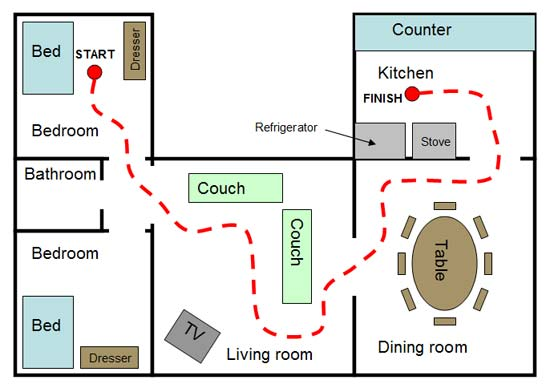
\includegraphics[width=0.85\textwidth, height=0.70\textheight]{figures/planning01.jpg}
%%%prolog/scale=0.47
%\label{fig_nos_estados}
\caption{\textit{A fome no meio da noite!}}
\end{figure}

%\framebreak

\end{frame}


\begin{frame}[fragile]
\frametitle{Exemplos do que é planejamento ...}

\begin{figure}[!htb]
\centering
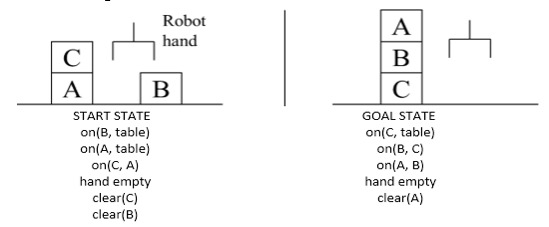
\includegraphics[width=0.850\textwidth, height=0.650\textheight]{figures/mundo_dos_blocos01.jpg}
%%%prolog/scale=0.47
%\label{fig_nos_estados}
\caption{O \textit{mundo dos blocos}}
\end{figure}

%\framebreak

\end{frame}


\begin{frame}[fragile]
\frametitle{Espaço de Estados}

\begin{figure}[!htb]
\centering
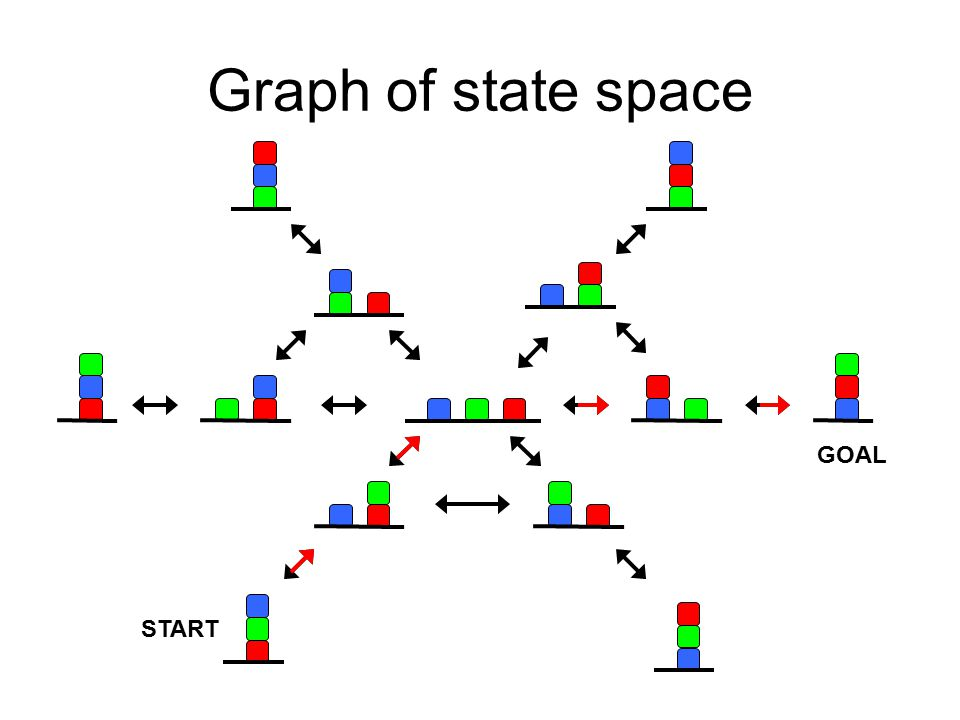
\includegraphics[width=0.7\textwidth, height=0.70\textheight]{figures/mundo_dos_blocos02.jpg}
%%%prolog/scale=0.47
%\label{fig_nos_estados}
\caption{O espaço de estados do \textit{mundo dos blocos} $\times$ ações}
\end{figure}

%\framebreak

\end{frame}



\begin{frame}[fragile, allowframebreaks=0.9]
\frametitle{Elementos de um  Planejador -- Vocabulário}

%%%%\textcolor{red}{PAREI AQUI}

\begin{itemize}
 \item \underline{Plano}: uma sequência ordenada de ações, 
 criada incrementalmente a partir do estado inicial\\
Ex. posições das peças de um jogo\\
$$S_1 < S_2 < ... < S_n$$
 
  \item \underline{Ambiente}: onde um programa--agente vai receber entradas em um determinado
  estado e atuar com uma ação apropriada

  \item  \underline{Estados}:   descrição completa de possíveis estados atingíveis\\
  Problema: quanto aos estados não-previstos, inacessíveis?

  \item  \underline{Estado inicial}: um estado particular onde nosso programa--agente
  inicia a sua busca
  
  \item \underline{Objetivos}: estados desejados que o programa--agente precisa alcançar,
  isto é, um dos \textit{estados finais} desejados

  \item  \underline{Percepções}: cheiro, brisa, luz, choque,
  som, posições ou coordenadas, vizinhanças, etc

  \item \underline{Ações}: provocam modificações entre os estados corrente e sucessor\\
  Exemplos: avançar para próxima célula, girar 90 graus à direita ou à esquerda
pegar um objeto, atirar na direção do alvo, etc
 
 \item \underline{Operadores}: vocabulário ou repertório de atuações atômicas do que o agente pode fazer.\\
 Exemplos: $pegar(X)$, $mover\_de(X,Y)$, $levantar(X)$, $livre(X)$, etc
 
 \item Uma eventual confusão: \textcolor{magenta}{\textbf{uma ação é um conjunto de um ou mais operadores}},
 e ainda, \textcolor{magenta}{\textbf{a ação é condicional}}. 
 A ação só é disparada se as condições de pré-requisitos forem 
 satisfeitas.
 
 \item \underline{Heurística}: alguma função que  indica o progresso sobre os estados
 não visitados e sua convergência para uma finalização do plano
 
 
\end{itemize}

\end{frame}



\begin{frame}[fragile, allowframebreaks=0.9]
  \frametitle{O Problema Exemplo}

\begin{figure}[!htb]
\centering
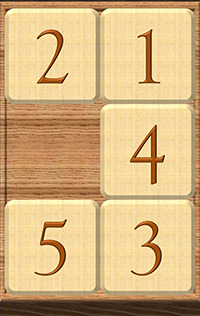
\includegraphics[width=.3\textwidth, height=0.40\textheight]{figures/puzzle_2x3_01.jpg}
%%%prolog/scale=0.47
%\label{fig_nos_estados}
\caption{Um quebra-cabeça ($2\times 3$ ou $3\times 2$) \textit{simplificado} do conhecido $3\times 3$}
\end{figure}


\framebreak
\begin{figure}[!htb]
\centering
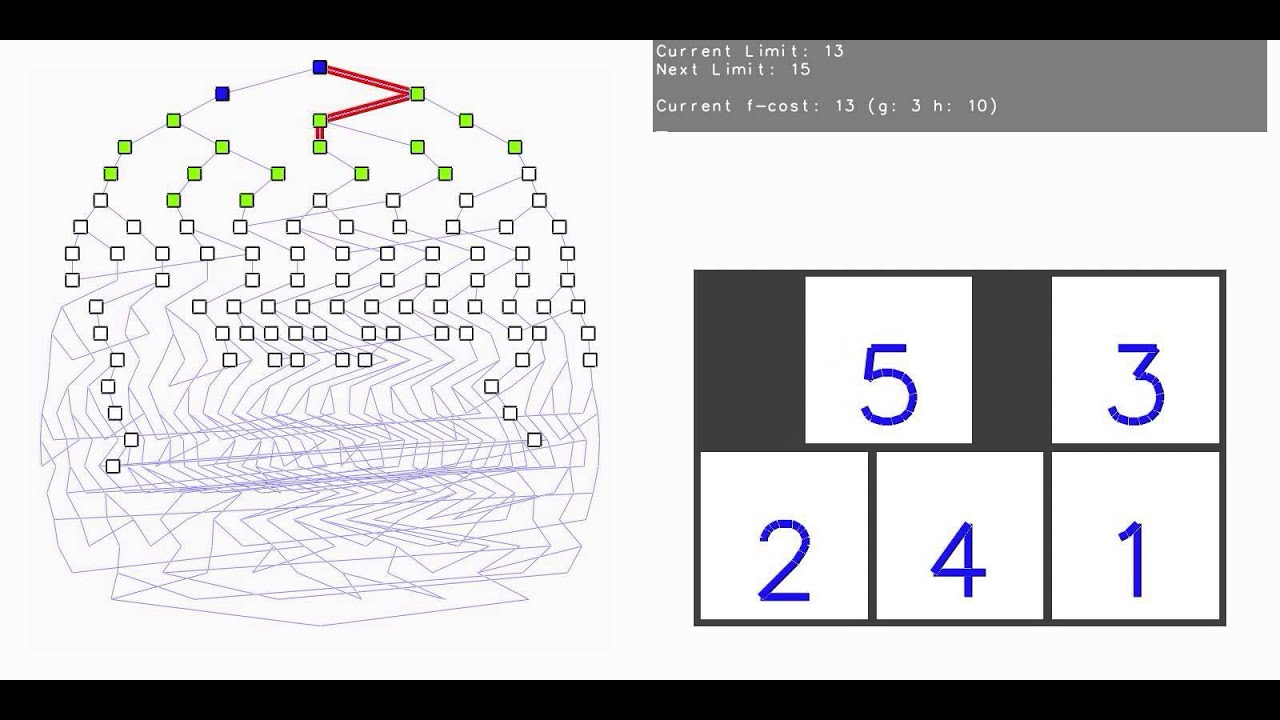
\includegraphics[width=.75\textwidth, height=0.65\textheight]{figures/puzzle_2x3_02.jpg}
%%%prolog/scale=0.47
%\label{fig_nos_estados}
\caption{Sim, \textit{simplificado} mas não muito!}
\end{figure}

\end{frame}

\begin{frame}[fragile, allowframebreaks=0.9]
 \frametitle{Partes do  código comentado}


\begin{footnotesize}
\begin{verbatim}
/*
A  B  C 
D  E  F
*/

%%%%%%%%%
%   1 5 %
% 4 3 2 %
%%%%%%%%%

import datetime.
import planner.
\end{verbatim}
\end{footnotesize}

\begin{center}
\textbf{\textcolor{red}{Atenção quanto a modelagem do problema, as 3 primeiras posicões da lista
correspondem a linha superior (A .. C), e as 3 últimas, a linha inferior (D .. F).}
}
\end{center}

\framebreak

\begin{footnotesize}
\begin{verbatim}
index(-)
estado_inicial( [0,1,5,4,3,2]  ).
%%%%%%%%%%%%%==> A,B,C,D,E,F

%% funcao final do planner
final( [1,2,3,4,5,0] ) => true .
%%%%==> A,B,C,D,E,F
%% pode ter uma condicional de parada

\end{verbatim}

\end{footnotesize}
\framebreak

\begin{footnotesize}
\begin{verbatim}
% Up <-> Down
/* Descrevendo as possiveis acoes para o planner */
action([A,B,C, D,E,F], S1, Acao, Custo_Acao ) ?=>
    Custo_Acao = 1,
    ( A == 0 ),  %% conj. condicoes
    S1 = [D,B,C, 0,E,F], 
    Acao = ($up(D),S1). %%a acao + estado modificado

action([A,B,C, D,E,F], S1, Acao, Custo_Acao ) ?=>
    Custo_Acao = 1,
    (A == 0 ),  %% conj. condicoes
    S1 = [0,B,C, A,E,F],
    Acao = ($dow(A),S1). %%a acao + estado modificado
.........................................................
\end{verbatim}
\end{footnotesize}

\framebreak


\begin{footnotesize}
\begin{verbatim}
% Left <-> Right
action([A,B,C, D,E,F], S1, Acao, Custo_Acao ) ?=>
    Custo_Acao = 1,
    (A == 0),  %% conj. condicoes
    S1 = [B,0,C, D,E,F],
    Acao = ($left(B), S1). %%a acao + estado modificado
    
action([A,B,C, D,E,F], S1, Acao, Custo_Acao ) ?=>
    Custo_Acao = 1,
    (B == 0),  %% conj. condicoes
    S1 = [0,A,C, D,E,F],
    Acao = ($right(A), S1). %%a acao + estado modificado
.........................................................
\end{verbatim}

\end{footnotesize}
\framebreak

\begin{footnotesize}
\begin{verbatim}
main  ?=>  
    estado_inicial( Q ),
    best_plan_unbounded( Q , Sol_Acoes), 
    println(sol = Sol_Acoes),
        
    printf("\n Estado Inicial: "),
    w_Quadro( Q ), 
    w_L_Estado( Sol_Acoes ), 
    Total := length(Sol_Acoes) ,
    Num_Movts := (Total -1) ,
    printf("\n Inicial  (estado): %w ", Q),
    printf("\n Total de acoes: %d", Total), 
    printf(" \n =========================================\n ")
    %%% fail ou false: descomente para multiplas solucoes
    .
 main => printf("\n Para uma solução .... !!!!" ) .
\end{verbatim}

\end{footnotesize}

\end{frame}



\begin{frame}[fragile]
 \frametitle{O código}

\begin{itemize}
  \item Acompanhar as explicações do código de:\\
\url{https://github.com/claudiosa/CCS/blob/master/picat/puzzle_2x3_planner.pi}

  \item Confira a execuç\~ao
\end{itemize}
\end{frame}


\begin{frame}[fragile, allowframebreaks=0.9]
 \frametitle{Parte da Saída}

\begin{footnotesize}
\begin{verbatim}
[ccs@gerzat picat]$ picat puzzle_2x3_planner.pi 
sol = [(left(1),[1,0,5,4,3,2]),(left(5),[1,5,0,4,3,2]),
(up(2),[1,5,2,4,3,0]),(right(3),[1,5,2,4,0,3]),(dow(5),[1,0,2,4,5,3]),
(left(2),[1,2,0,4,5,3]),(up(3),[1,2,3,4,5,0])]

 Estado Inicial: 
 0 1 5
 4 3 2

Acao: left(1)
 1 0 5
 4 3 2

Acao: left(5)
 1 5 0
 4 3 2
\end{verbatim}
\end{footnotesize}

\framebreak
\begin{footnotesize}
\begin{verbatim}
.................................
Acao: left(2)
 1 2 0
 4 5 3

Acao: up(3)
 1 2 3
 4 5 0

 Inicial  (estado): [0,1,5,4,3,2] 
 Total de acoes: 7 
 =========================================
\end{verbatim}
\end{footnotesize}

\end{frame}



\begin{frame}[fragile]
 \frametitle{O módulo do \textit{planner} do Picat}

\begin{itemize}
  \item O que efetivamente voce precisa saber
  
  \pause
  \item Importar um módulo \\
   \textbf{\texttt{import planner.}}

   \pause
   \item O predicado: \textit{final}\\
    \textbf{\texttt{final(S,Plan,Cost) => Plan=[], Cost=0, final(S).}}
   
    \pause
    \item O predicado \textit{action}\\
    \textbf{\texttt{action(S,NextS,Action,ActionCost)}}

\end{itemize}
\end{frame}


\begin{frame}[fragile]
 \frametitle{O módulo do \textit{planner} do Picat}

\begin{itemize}

 \item A \textcolor{magenta}{\textbf{eficiência}} do planner do Picat se dá devido a sua combinação
       de técnicas: \textcolor{magenta}{busca em profundidade} (e variações) e \textcolor{magenta}{Programação
       Dinâmica (PD)} (uso do \textit{tabling})


  \pause 
  \item O núcleo de busca dos planejadores  disponíveis no Picat são de 2 tipos:
  \begin{enumerate}
    \item Usam um busca em profundidade com limites (\textit{Depth-Bounded Search})
    \item Usam um busca em profundidade ilimitada de recursos (\textit{Depth-Unbounded Search}) 
  \end{enumerate}
  
  \item Contudo, estes 2 tipos apresentam muitas variações e opções:\\
  \pause
  Sem escapatória $\Rightarrow $ consultar o manual do Picat (\textit{User Guide to Picat})
  
  \item No exemplo aqui apresentado: 
  \texttt{best\_plan\_unbounded(S,Plan)}   
\end{itemize}
\end{frame}




\begin{frame}[fragile]
\frametitle{Reflexões}


\begin{itemize}
  \item Planejamento resolve uma classe ampla de problemas\\
   Havendo necessidade de
    \textcolor{magenta}{\textbf{descobrir sequências ações}} $\Leftrightarrow$ \textcolor{violet}{Planejamento}

  \pause
  \item Em geral, estes problemas são importantes na indústria

  \pause
  \item Os modelos escritos em PDDL (\textit{Planning Domain Definition Language})
  facilmente portáveis para Picat
    \pause
  \item Sob um uso mais restrito, um modelo em PDDL é executado diretamente em Picat
    
  \pause
  \item Na próxima seção uma outra técnica de resolver problemas: \textbf{\underline{PR}}
\end{itemize}

\end{frame}

 % 9
 \section{Conclusões}
%%%%%%%%%%%%%%%%%%%%%%%%%%
\begin{frame}[fragile]
\frametitle{Conclusões}
\begin{minipage}{0.47\textwidth}
    \begin{itemize}
        \item O que foi visto
        \item O que tem a ser feito
        \item Oportunidades
    \end{itemize}
\end{minipage}
\begin{minipage}{0.5\textwidth}
\begin{figure}[ht!]
\begin{center}

\includegraphics[width=1.2\textwidth, height=0.40\textheight]{figures/logo_picat_alex.jpg}
\end{center}
\end{figure}
\end{minipage}
\end{frame}
%%%%%%%%%%%%%%%%%%%%%%%%%%
\begin{frame}[fragile]

    \frametitle{Conclusões}

    \begin{itemize}
      \item Picat é jovem  $\approx$ 2013
      \pause
      \item Uma evolução ao Prolog após seus mais de 40 anos de existência e sucesso!
      \pause
      \item Sua sintaxe é moderna e intuitiva
      \pause
      \item Código aberto, multi-plataforma e repleta de possibilidades (sistemas embarcados, combinatória,
      SO, escalonamentos, planejamento etc) $\Rightarrow$ NP's completos em geral
%      \pause
%      \item Uso para fins diversos
      \pause
      \item Muitas bibliotecas específicas prontas: CP (PR), SAT, Planner, etc
      \pause
      \item A sintaxe de PR exige um pouco mais do programador
      \pause
      \item Dúvidas: o guia do usuário, livro do Hakan e o Fórum de discussão do Picat

    \end{itemize}
\end{frame}


%%%%%%%%%%%%%%%%%%%%%%%%%%

\subsection{Ficou Faltando}
\begin{frame}[fragile]

    \frametitle{Ficou Faltando:}

    \begin{itemize}
      \item Uso do \texttt{debug} e \texttt{trace} (cansativo -- uma oportunidade) $\Rightarrow$ \textcolor{magenta}{\textbf{Pendência resolvida!}} 

     \pause
     \item Explorar uso dos \textit{solvers} de PO (fácil)

      \pause
      \item Explorar a criação e  uso de módulos  (mais fácil ainda)



    \end{itemize}
\end{frame}



\subsection{Dicas de Programação}
\begin{frame}[fragile] 

    \frametitle{Dicas de Programação:}

    \begin{itemize}
      \item Use o interpretador e o compilador concomitamente. O interpretador
      sempre acusa \textit{warnings} etc. O modo compilado na console não apresenta
      alguns \textit{warnings}. Efeito \textit{cascata} de erro ...

      \pause
      \item No modo interpretado, cada linha de código pode ser testada isoladamente,
      assim, o efeito global desta é restrita. Qualquer erro ou falha é rapidamente
      detectada.

       \pause
      \item Consulte o manual do usuário \textit{on-line} em \textit{html}, 
      mantido pelo Alexandre Gonçalves -- UFSC
      \url{http://retina.inf.ufsc.br/picat_guide}


      \pause
      \item Consulte o site do Picat e dos grandes mestres Hakan, Neng-Fa, Roman Barták, 
      Sergii Dymchenko, etc

      \pause
      \item Inscreva-se no fórum e consulte o Guia do Usuário (tudo em inglês)


    \end{itemize}
\end{frame}



\subsection{Agradecimentos}
\begin{frame}[fragile]

    \frametitle{Agradecimentos}

    \begin{itemize}
      \item Muito obrigado a voce!
      \pause
      \item Algumas pessoas que deram opiniões neste material 
            e me incentivaram a terminá-lo 
            
      \pause
      \item  Em especial a minha esposa: Maria Luiza
  
      \pause
      \item Claudio Cesar de Sá
     \item Contacto: 
     \begin{description}
          \item[\Letter \/] \url{claudio.sa@udesc.br}
          \item[\Letter \/] \url{claudio@colmeia.udesc.br}
     \end{description}


    \end{itemize}
\end{frame}



\begin{frame}[fragile]
  \frametitle{Finalizando ...}


\begin{minipage}{0.47\textwidth}

\begin{Large}
\textbf{\textcolor{magenta}{... espero que\\ tenham gostado\\ e obrigado!}}
\end{Large}

\end{minipage}
\begin{minipage}{0.5\textwidth}
\begin{figure}[ht!]
\begin{center}

\includegraphics[width=1.2\textwidth, height=0.40\textheight]{figures/logo_picat_alex.jpg}
\end{center}
\end{figure}
\end{minipage}

\end{frame}
					
 % 11
\end{document}
